This section presents and examines the results of the modeling outlined in the previous section. $\S$ \ref{Par_stress} shows the effects of changing important input parameters, such as the temperature, on a simulated spectrum of Gallium-69.  

\section{Initial Test}
As a first test, this Fig. \ref{comp} presents a comparison between a measured spectrum of Gallium-69 and a simulated spectrum generated using the parameters given in Tables \ref{hyperfinecoeff} and \ref{othercoeff}.

\begin{figure}[h]
\centering
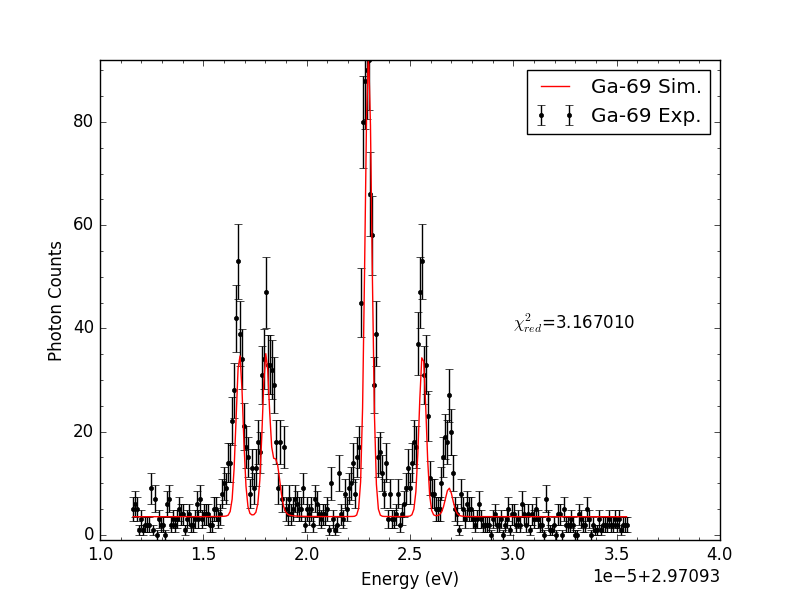
\includegraphics[width = 0.8\textwidth]{Graphics/Ga-69-vs-sim.png}
\caption[Comparison between a measured spectrum of Gallium-69 and a spectrum simulated.]{\small Comparison between a measured spectrum of Gallium-69 and a spectrum simulated using the parameters given in in Tables \ref{hyperfinecoeff} and \ref{othercoeff}. A reduced $\chi^2$ statistic of 3.167010 is also reported as a measure of accuracy between the simulation and data. A clear difference peak widths of the two spectra can be seen. }
\label{comp}
\end{figure}

\begin{table}[h]
\centering
\begin{tabular}{c c c c}\hline
$A_u$ (MHz)&$A_l$ (MHz)&$B_u$ (MHz)&$B_l$ (MHz)\\ \hline
1070.908128 & 188.512676 & 0 & 68.333737\\ \hline \\
\end{tabular}
\caption[Hyperfine parameters used in the simulation of the spectrum of Gallium-69.]{\small Hyperfine parameters used in the simulation of the spectrum of Gallium-69.\citep{gapap}}
\label{hyperfinecoeff}
\end{table}

\begin{table}[h]
\centering
\begin{tabular}{c c c}\hline
Temperature (K)&Power (mW)&CEC-LCR Dist. (m)\\ \hline
300 & 1.0 & 0.40\\ \hline \\
\end{tabular}
\caption[Other parameters required for the simulation of a hyperfine spectrum.]{\small Other parameters required for the simulation of a hyperfine spectrum. The power and CEC-LCR distance are measured quantities, while the temperature is estimated.}
\label{othercoeff}
\end{table}

A distinct difference in the peak widths between the simulated and measured spectra can be seen in Fig. \ref{comp}, where the simulated spectrum has narrower peaks than the measured spectrum. Since the temperature is merely an estimate based on the cooling methods used to bunch the atoms, it is possible that the estimated temperature is inaccurate. Fig. \ref{chi_temp} shows the reduced $\chi^2$ statistic as a function of the temperature used in the simulation. The estimated temperature of 300 K is lower than the temperature that produces the lowest reduced $\chi^2$ value, occurring at $\sim$910 K.
\begin{figure}[h]
\centering
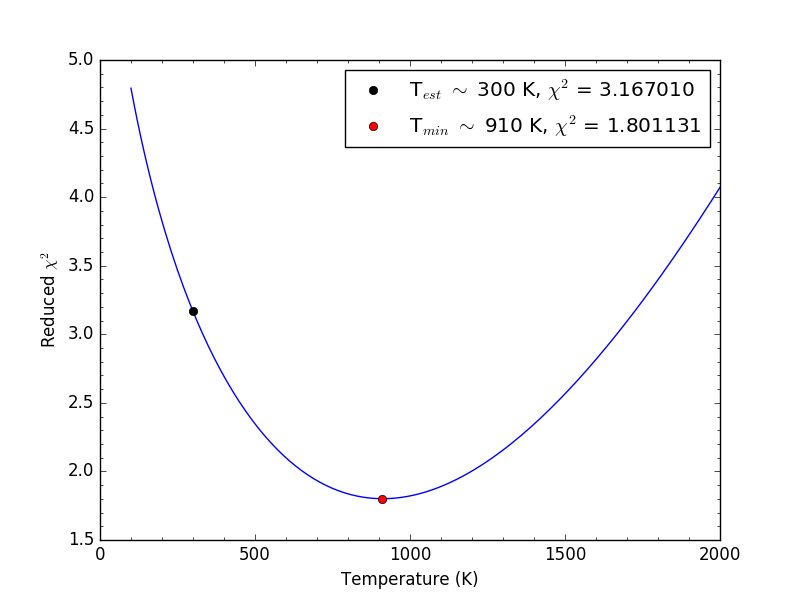
\includegraphics[width=0.8\textwidth]{Graphics/temp_chi.png}
\caption[Reduced $\chi^2$ statistic as a function of the temperature used in the simulation of a Gallium-69 hyperfine spectrum.]{\small The reduced $\chi^2$ statistic as a function of the temperature used in the simulation of a Gallium-69 hyperfine spectrum. The estimated temperature of 300 K is shown, as well as the temperature at which a minimum in the $\chi^2$ value occurs, $\sim$ 910 K.}
\label{chi_temp}
\end{figure}
\section{Temperature, CEC-LCR Distance and Power}
\label{Par_stress}
In this section, the effects of changing the temperature of the beam, the distance between the CEC and the LCR, and  the laser power  are shown and discussed. 

\subsection{Temperature}
The temperature of the atoms as they interact with the laser is expected to affect the widths of the peaks in the resulting hyperfine spectra. Eq. \ref{temp_width} describes the effects of temperature on the Gaussian contribution to the width of a Voigt profile. Fig \ref{temp_comp} shows the effects of temperature on a simulated spectrum of Gallium-69. As the temperature increases doppler broadening begins to dominate the width of the peaks and the hyperfine structure of the spectrum is diluted. 
\begin{figure}[h!]
\begin{center}
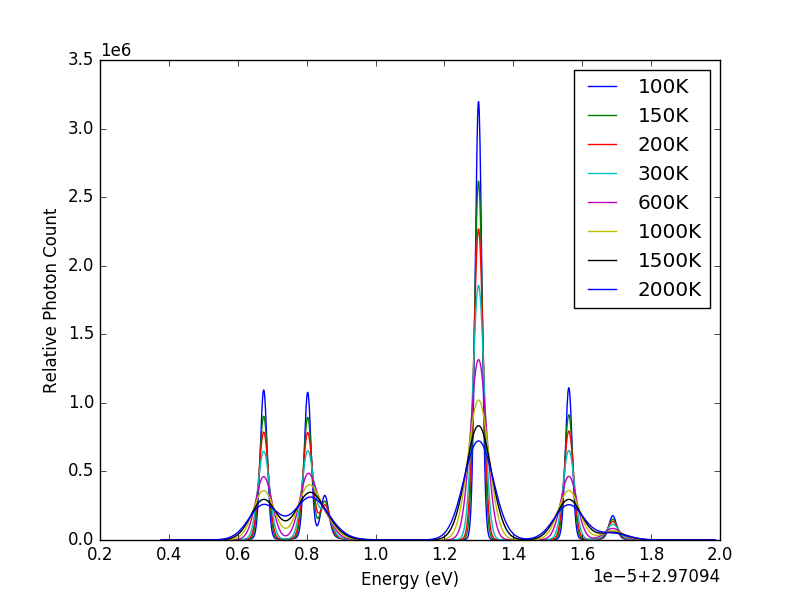
\includegraphics[width = 0.8\textwidth]{Graphics/temp_comparison.png}
\end{center}
\caption[The effects of the temperature on the hyperfine spectrum of Gallium-69.]{\small The effects of the temperature on the hyperfine spectrum of Gallium-69. As the temperature of the atoms increases, the doppler contribution to the width of the peaks increases. At sufficiently high temperatures ($\approx 2.0 \times 10^3$ K), the hyperfine structure of the atom begins to smooth out.}
\label{temp_comp}
\end{figure}

\subsection{CEC-LCR Distance}
Eq.\ref{prob_unchanged} inversely depends on the distance between the CEC and the LCR. The likelihood of an atom reaching the LCR in its original ground state decreases as the CEC-LCR distance increases. Conversely, this likelihood increases as the CEC-LCR distance decreases. Fig \ref{CEC-LCR} shows the effects of changing this distance on a simulated Gallium-69 spectrum. Between 0.1 and 1.0 m, there is no discernible difference between the simulated spectra. As the distance is increased to 2 and then 5 m, optical pumping begins to take effect, with the right-most peak being nearly pumped out at 5 m. 
\begin{figure}[h!]
\begin{center}
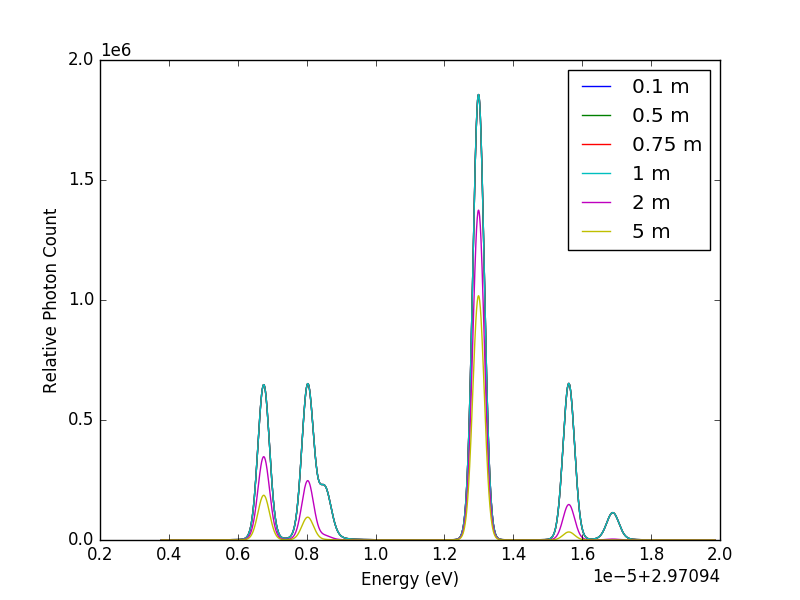
\includegraphics[width=0.8\textwidth]{Graphics/dist_comparison.png}
\end{center}
\caption[The effects of changing the CEC-LCR distance on a simulated spectrum of Gallium-69.]{\small The effects of changing the CEC-LCR distance on a simulated spectrum of Gallium-69. As the distance increases, optical pumping begins to have a larger effect. At 5 m, the central peak begins to completely dominate the spectrum at the expense of the smaller peaks near 1.5 and 4 $\times 10^{-3}$+2.9709512 eV.}
\label{CEC-LCR}
\end{figure}

\subsection{Laser Power}
The power of the laser is the most important parameter when simulating the effects of optical pumping on a hyperfine spectrum. This sections first shows the behavior of the model as the power is changed. Figures \ref{power1-40} and \ref{power50-100} show how a simulated spectrum of Gallium-69 changes as the power of the exciting laser is increased from 1.0 to 100 mW. 

\begin{figure}[h!]
\begin{center}
\begin{subfigure}{0.75\textwidth}
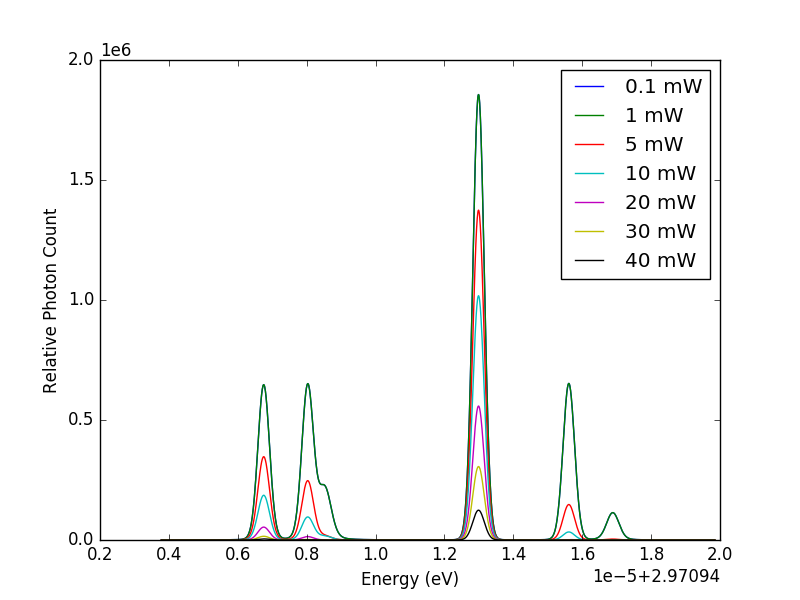
\includegraphics[width = \textwidth]{Graphics/Power_comparison(1-40).png}
\caption[The effects of the power of the exciting laser on a simulated Gallium-69 spectrum.]{\small The effects of the power of the exciting laser on a simulated Gallium-69 spectrum are shown above. As the power of the laser is increased, certain transitions become less likely with respect to others, changing the relative intensities of the peaks. }
\label{power1-40}
\end{subfigure}

\begin{subfigure}{0.75\textwidth}
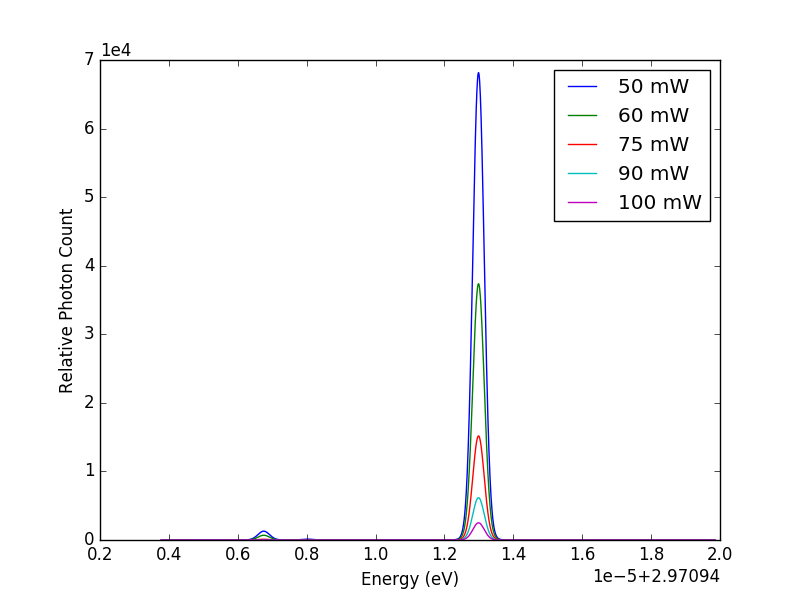
\includegraphics[width = \textwidth]{Graphics/Power_comparison(50-100).png}
\caption[Continuation of Fig \ref{power1-40}]{\small Increasing the power of the laser causes optical pumping to have a greater effect on the resulting spectrum. Peaks corresponding to transitions that have lower likelihoods of reaching the LCR in their original ground states have relative intensities that decrease with respect to the more resilient peaks. }
\label{power50-100}
\end{subfigure}
\end{center}
\end{figure}

\pagebreak
\subsubsection{Rubidium-87}
In a recent experimental run at TRIUMF, a hyperfine spectrum of Rubidium-87 (I = 1.5, $J_e$ = 1.5, $J_g$ = 0.5) was examined as the power of the exciting laser was changed. Below are the results of the run, compared to the spectra predicted by the algorithm described in the previous chapter.

\begin{figure}[h]
    \centering
    \begin{subfigure}[b]{0.49\textwidth}
        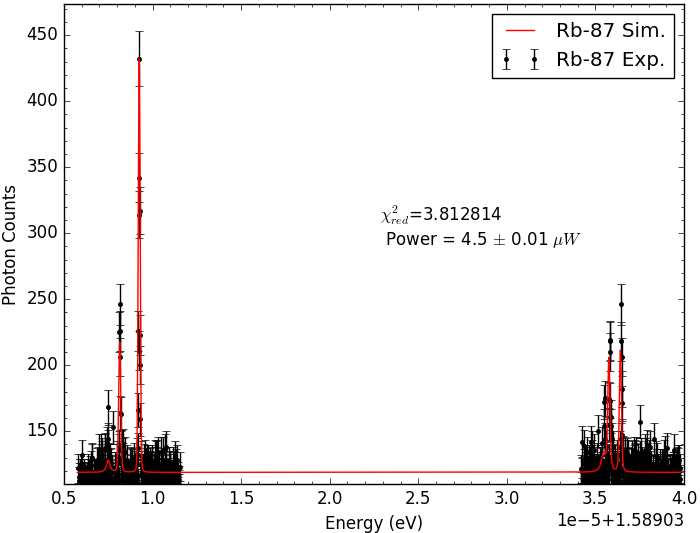
\includegraphics[width=\textwidth]{Graphics/100_101.png}
        \caption{}
    \end{subfigure}
    \begin{subfigure}[b]{0.49\textwidth}
        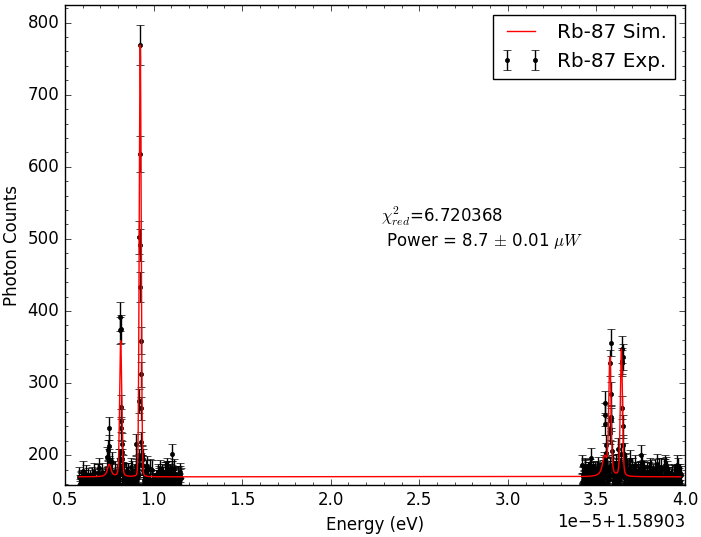
\includegraphics[width=\textwidth]{Graphics/098_099.png}
        \caption{}
        \label{}
    \end{subfigure}
    
  	\begin{subfigure}[b]{0.49\textwidth}
        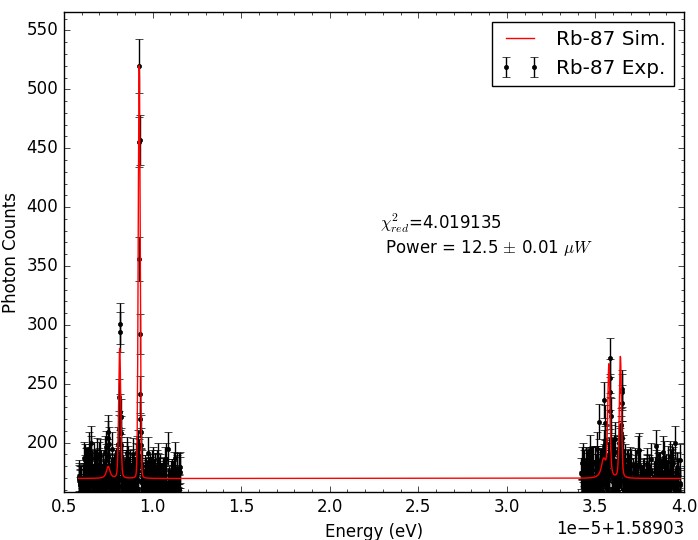
\includegraphics[width=\textwidth]{Graphics/119_120.png}
        \caption{}
    \end{subfigure}
    \begin{subfigure}[b]{0.49\textwidth}
        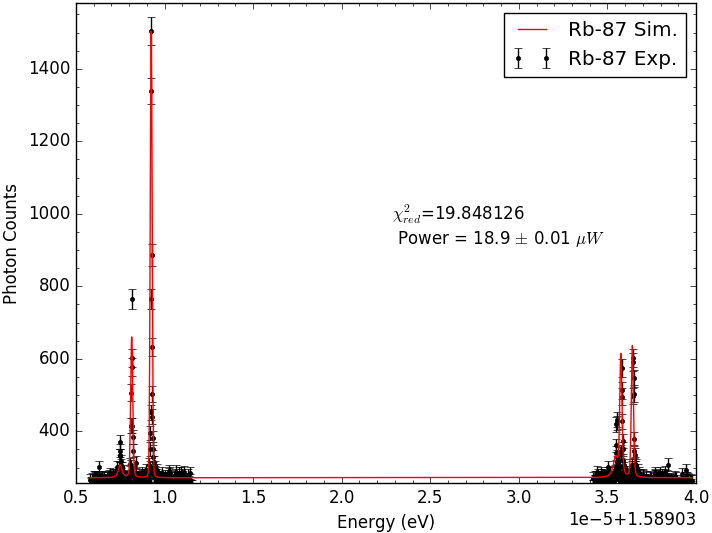
\includegraphics[width=\textwidth]{Graphics/096_097.png}
        \caption{}
        \label{}
    \end{subfigure}
    \caption[Comparison between the simulated and measured hyperfine spectra of Rubidium-87 for different laser powers.]{\small Comparison between the simulated (red) and measured (black) hyperfine spectrum of Rubidium-87 for laser power: (a) 4.5 $\mu W$ (b) 8.7 $\mu W$ (c) 12.5 $\mu W$ (d) 18.9 $\mu W$. The lack of data between the two groups of peaks is due to the method of scanning used. To reduce the collection time required, only the regions where peaks were expected were scanned. Also shown are the reduced $\chi^2$ values for each comparison. The simulated spectra tend to exaggerate the effects of optical pumping, exemplified by the predicted height of the left-most peak. In each case, this peak is much lower than the corresponding peak in the measured spectrum. }
    \label{power4-18}
\end{figure}
Fig. \ref{chi_vs_power} shows the performance of the model when compared to the Rubidium-87 spectra. The reduced $\chi^2$ statistic is reported for each Rubidium spectrum and is plotted as a function of the laser power. As a general trend, the model accuracy decreases as the power increases. Examining the comparisons between the predicted and measured spectra of Rubidium-87, a discrepancy between the expected and measured height of the lowest energy peak, located at $\sim$ 0.75e-5+1.58903 eV, is present across all laser powers, indicating that the model overestimates the effects of optical pumping for this transition ($F_e$ = 1 $F_g$ = 0).

\begin{figure}[t!]
	\centering
    \begin{subfigure}[b]{0.49\textwidth}
        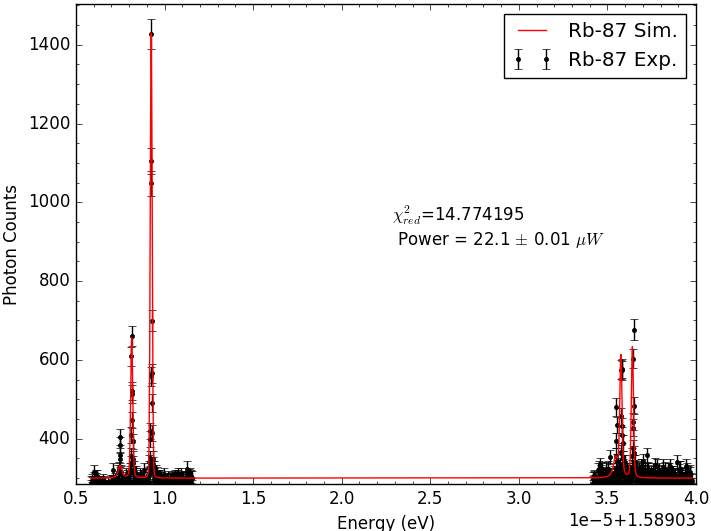
\includegraphics[width=\textwidth]{Graphics/107_108.png}
        \caption{}
    \end{subfigure}
    \begin{subfigure}[b]{0.49\textwidth}
        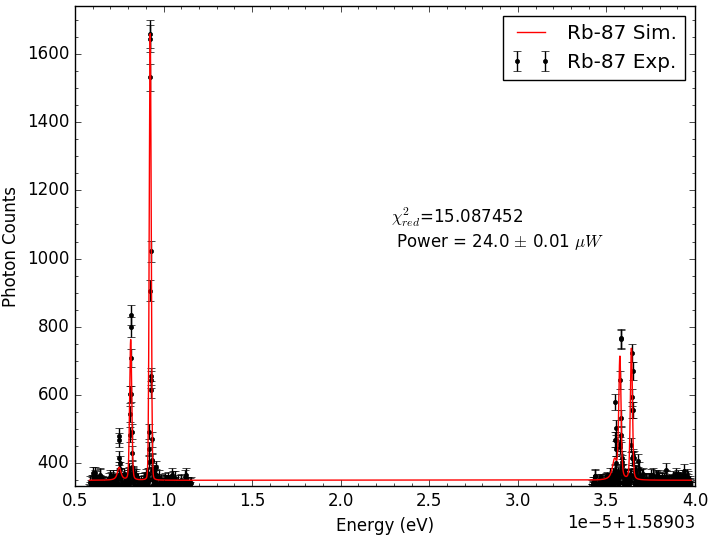
\includegraphics[width=\textwidth]{Graphics/094_095.png}
        \caption{}
        \label{}
    \end{subfigure}

    \begin{subfigure}[b]{0.49\textwidth}
        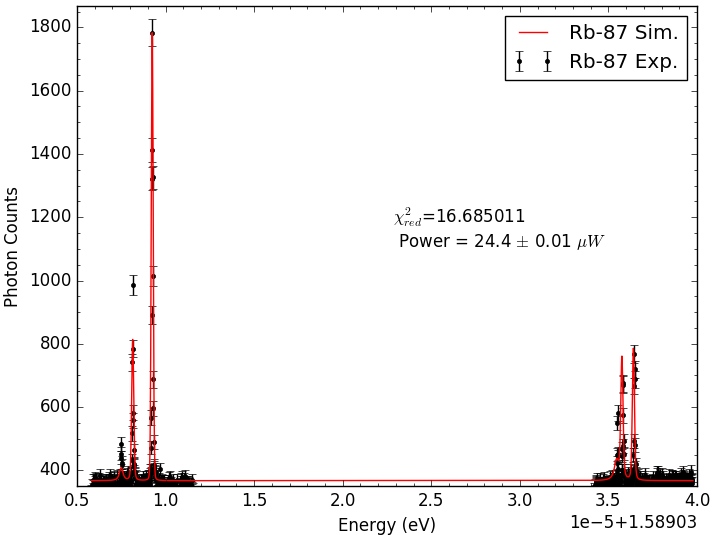
\includegraphics[width=\textwidth]{Graphics/121_122.png}
        \caption{}
    \end{subfigure}
    \begin{subfigure}[b]{0.49\textwidth}
        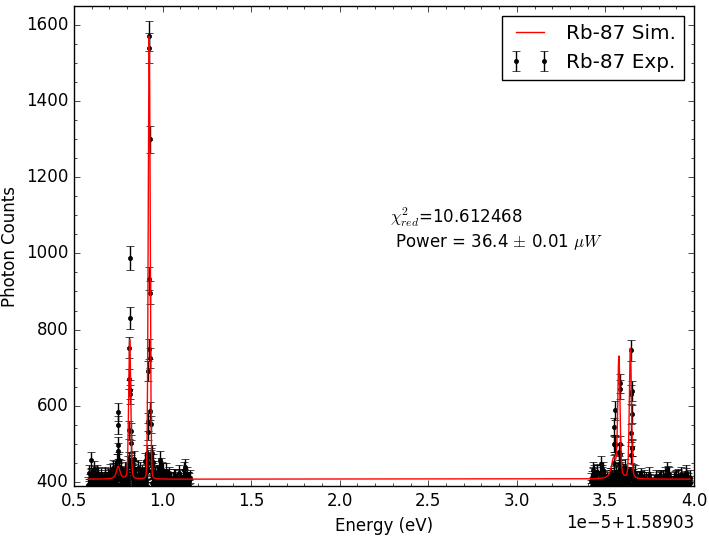
\includegraphics[width=\textwidth]{Graphics/111_112.png}
        \caption{}
        \label{}
    \end{subfigure}
    \caption[Continuation of Fig. \ref{power4-18}.]{\small Continuing from Fig. \ref{power4-18}, a comparison between the simulated (red) and measured (black) hyperfine spectrum of Rubidium-87 for laser power: (a) 22.1 $\mu W$ (b) 24.0 $\mu W$ (c) 24.4 $\mu W$ (d) 36.4 $\mu W$. Also shown are the reduced $\chi^2$ values for each comparison. Following the trend shown in the previous spectra, the simulated spectra tend to exaggerate the effects of optical pumping, shown by the discrepancy between the predicted and measured heights of the left-most peak. In each case, this peak is lower than the corresponding peak in the measured spectrum. }
\label{power22-36}
\end{figure}
\pagebreak
\begin{figure}[h]
	\centering
    \begin{subfigure}[b]{0.49\textwidth}
        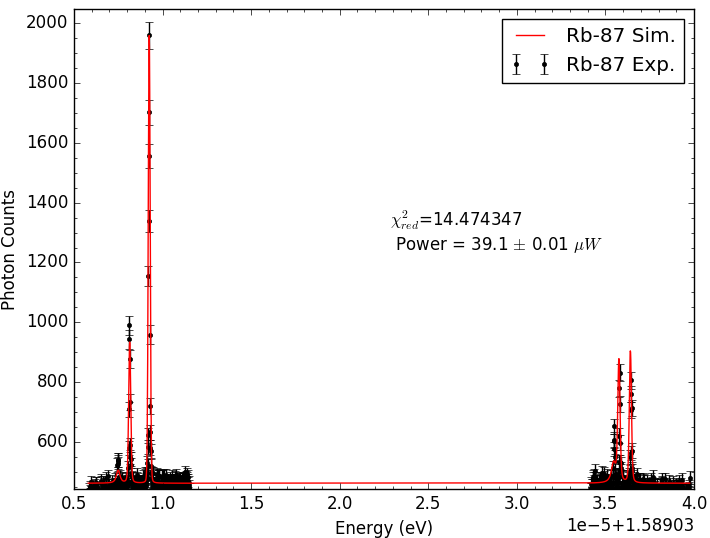
\includegraphics[width=\textwidth]{Graphics/113_114.png}
        \caption{}
        \label{}
    \end{subfigure}
    \begin{subfigure}[b]{0.49\textwidth}
        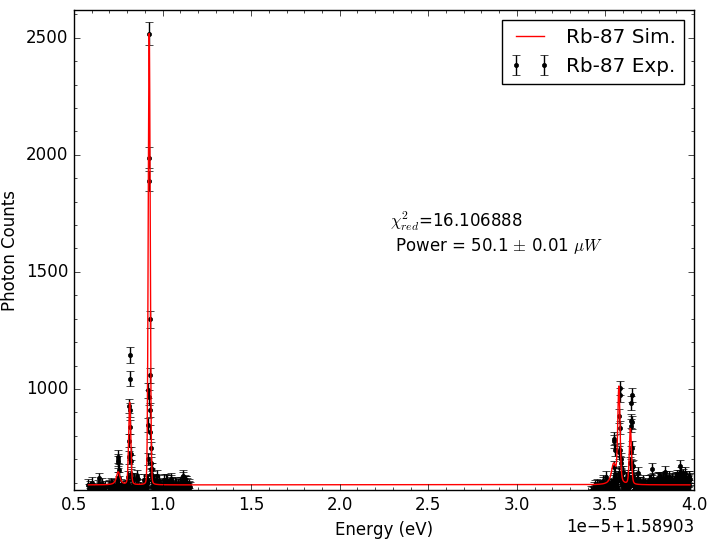
\includegraphics[width=\textwidth]{Graphics/115_116.png}
        \caption{}
    \end{subfigure}
    
    \begin{subfigure}[b]{0.49\textwidth}
        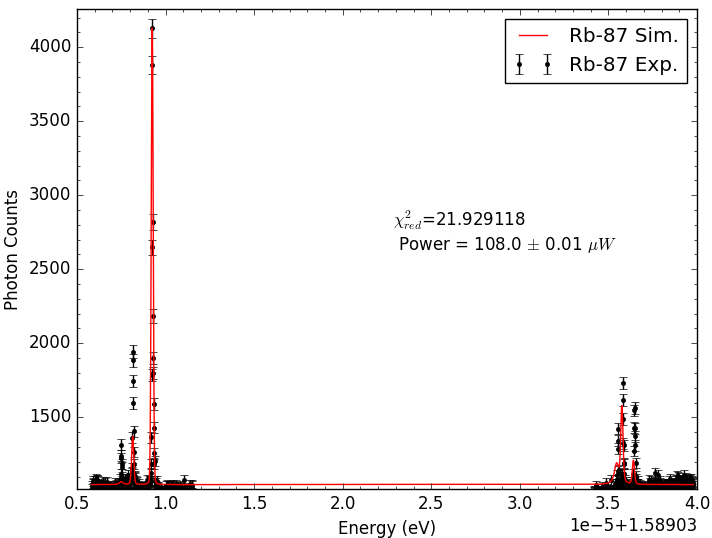
\includegraphics[width=\textwidth]{Graphics/117_118.png}
        \caption{}
        \label{}
    \end{subfigure}
    \begin{subfigure}[b]{0.49\textwidth}
        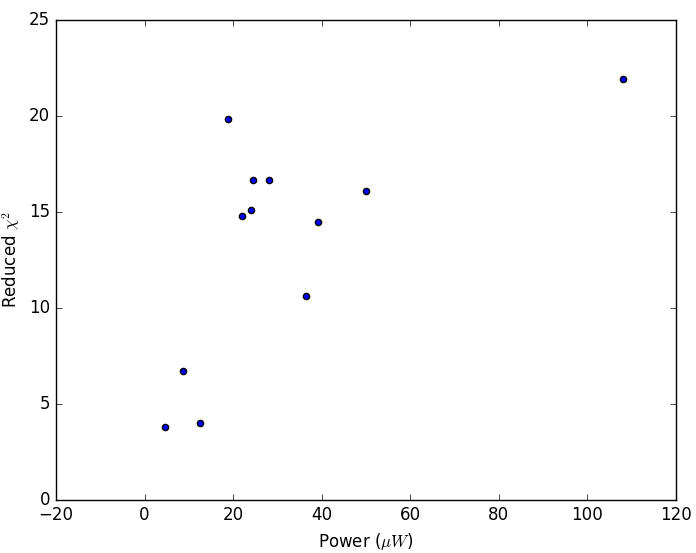
\includegraphics[width=\textwidth]{Graphics/chi-v-power.png}
        \caption{}
        \label{chi_vs_power}
    \end{subfigure}
    \caption[The final set of spectra exploring the effect of the laser power on the hyperfine spectrum on Rubidium-87.]{\small The final set of spectra exploring the effect of the laser power on the hyperfine spectrum on Rubidium-87, compared to the spectra predicted by the method outlined in Chapter \ref {Op_pump} The laser powers are: (a) 39.1 $\mu W$ (b) 50.1 $\mu W$ (c) 108.0 $\mu W$. Also shown are the reduced $\chi^2$ values for each comparison. (d) shows the reduced $\chi^2$ statistic as a function of the power of the exciting laser for the Rubidium-87 experimental run. As the power increases, the model reproduces the spectrum less accurately, as shown by the increase in the value of the $\chi^2$ statistic. }
\label{power39-108}
\end{figure}
